\documentclass{article}

\usepackage[preprint]{nips_2018}
% to avoid loading the natbib package, add option nonatbib:
% \usepackage[nonatbib]{nips_2018}

\usepackage[utf8]{inputenc} % allow utf-8 input
% \usepackage[T1]{fontenc}    % use 8-bit T1 fonts
\usepackage{hyperref}       % hyperlinks
\usepackage{url}            % simple URL typesetting
\usepackage{booktabs}       % professional-quality tables
\usepackage{amsfonts}       % blackboard math symbols
\usepackage{nicefrac}       % compact symbols for 1/2, etc.
\usepackage{microtype}      % microtypography
\usepackage{amsmath}
\usepackage{mathtools}
\usepackage{float}
\usepackage{graphicx}
\usepackage{algorithm}
\usepackage{algpseudocode}
\usepackage{cleveref}       % this package must be loaded at the last
\usepackage{subcaption}
\usepackage{enumitem}

\DeclareMathOperator*{\argmax}{argmax}
\newlist{steps}{enumerate}{1}
\setlist[steps, 1]{label = Step \arabic*:}

\title{Lab1 Report}

\author{
  Chun Hung Lin \\
  \texttt{chlin3@kth.se}
  \And
  Yini Yang \\
  \texttt{yiniy@kth.se} \\
  \texttt{199504244188}
}

\begin{document}
\maketitle

% Quesiton 1
\section{Problem 1: The Maze and the Random Minotaur}

\subsection{Formulate the problem as an MDP}

This problem can be formulated as an MDP with finite horizon.

\textbf{State space:}

Here we use a pair of positions in the maze as a state. The state space $S$ can be described as follows:
$$ S = \{S_i=(x_p,y_p,x_m,y_m)|i=0,\cdots,3135\}, \quad x_p,x_m\in [0,6],\  y_p,y_m\in [0,7]$$
where $(x_p,y_p)$ refers to the position of the person, while $(x_m,y_m)$ is the position of the Minotaur.
Here we can divide this state space into four part:
$$ S = S_{\text{unavailable}}\cup S_{\text{available}}\cup S_{\text{dead}}\cup S_{\text{escape}}$$


where $S_{\text{unavailable}}=\{(x_p,y_p)\in \text{wall}\}$ refers to the states where the person is in the wall.
$S_{\text{dead}}=\{S_i|x_p=x_m,y_p=y_m\}$ corresponds to the states where the person and minotaur are in the same position.
$S_{\text{escape}}=\{S_i|(x_p,y_p)=exit,(y_p,y_m)\neq exit\}$ includes the states at which the person succeeds escaping.
And both $S_{\text{dead}}, S_{\text{escape}}$ are absorbing states.


\textbf{Action space:}
In this problem, the minotaur follows a random walk. The action space for the person is as below:

\begin{equation*}
  A=\{\textup{Up},\textup{Down},\textup{Left},\textup{Right},\textup{StandStill}\}
\end{equation*}

\textbf{Reward:}

The reward can be formulated as a function of $r: S\times A\rightarrow \mathbb{R}$.
\begin{equation*}
  r(s, :) =
  \begin{cases}
    -10  \quad &s\in S_{\text{escape}}\\
    1    \quad &s\in S_{\text{dead}} \\
    0    \quad &\textup{otherwise}
  \end{cases}
\end{equation*}

When the state is in $S_{escape}$, no matter what actions the person take, the reward will always be 10.
While the state is in $S_{dead}$, the punishment will be $-1$ for whatever actions.
For other available movement, there will be no reward or punishment.
% \newline

\textbf{Transition probability:}

For the person, the policy is deterministic. In other words, given the current position and the action, the next position of the person is deterministic.
So for the state transition, the uncertainty comes from the minotaur. Thus the transition probability can be formulated as follows:
% $$P_t(s_j|s_i,a)=\left\{\begin{aligned}
%   &\frac{1}{|\textup{Aja}(s_{i_M})|} \quad &s_{j_M}\in \textup{Aja}(s_{i_M}) \\
%   &1 \quad &S_i\in S_{dead}\cup S_{escape} \\
%   &0 \quad &\textup{otherwise}
% \end{aligned}\right.$$
\begin{equation*}
  P_t(s_j|s_i,a) =
  \begin{dcases}
    \frac{1}{|\textup{Adj}(s_{i_M})|}
        \quad &s_{j_M}\in \textup{Adj}(s_{i_M}) \\
    1   \quad &S_i\in S_{dead}\cup S_{\text{escape}} \\
    0   \quad &\textup{otherwise}
  \end{dcases}
\end{equation*}
where $s_{i_M}=(x_{i_m},y_{i_m})$ means the minotaur's position at state $i$, and $\textup{Adj}(s_{i_M})$ is the set of adjacent positions to $s_{i_M}$.
And when the environment has reached the absorbing state, it will always stay in this state.
% \newline

\textbf{Objective funcion:}

This MDP is under a finite time horizon $T$. Thus the objective function can be formulated as the total rewards obtained in $T$ steps:
\begin{equation*}
  G_T=\mathbb{E}_{\tau}\left\{\sum_{t=1}^T r_t(s_t,a_t)\right\}
\end{equation*}
where $\tau$ is the trajectory under a policy $\pi$

\subsection{Solve the problem for T=20}
One generated solution has been shown in Figure \ref{solution}.
The red arrows correspond to the person's route, while the blue ones refer to the minotaur's route.
In this solution, the person succeeds escaping when $t=17$.
\begin{figure}[h]
  \centering
  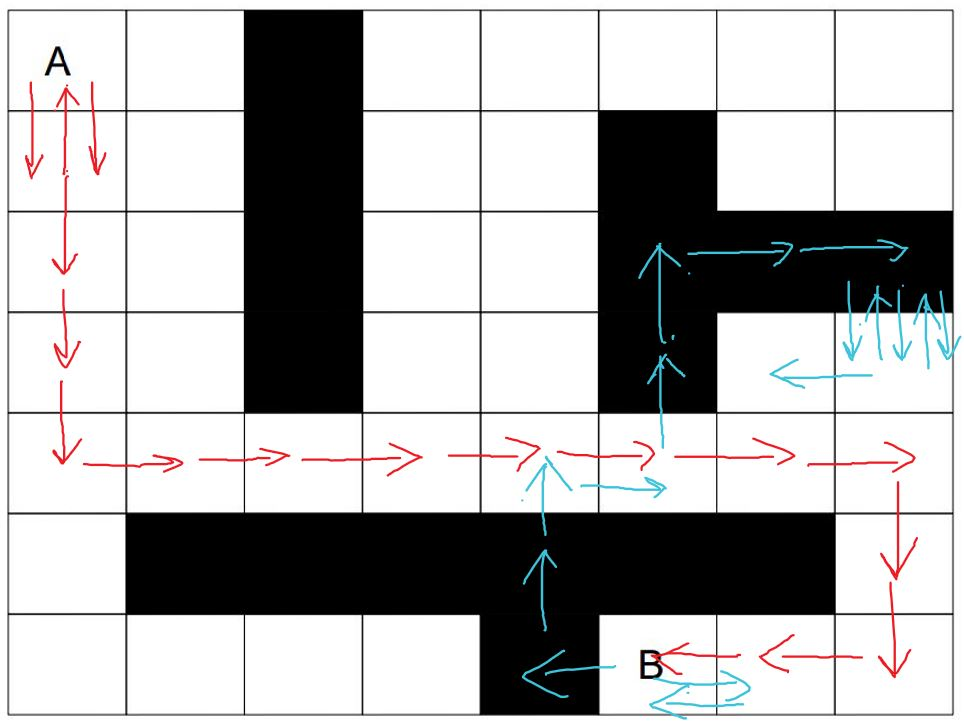
\includegraphics[scale=0.4]{solution.jpg}
  \caption{A generated solution for T=20. (Red trajectory: person, blue trajectory: minotaur.)}
  \label{solution}
\end{figure}

The maximal probability of exiting the maze has been estimated as a function of T. Here we consider both cases of whether the minotaur is allowed to stand still or not.
The results for $T\in [1,30]$ are shown in Figure \ref{fig:prob-getout-alive}.
\begin{figure}[H]
  \centering
  \begin{subfigure}{.5\textwidth}
    \centering
    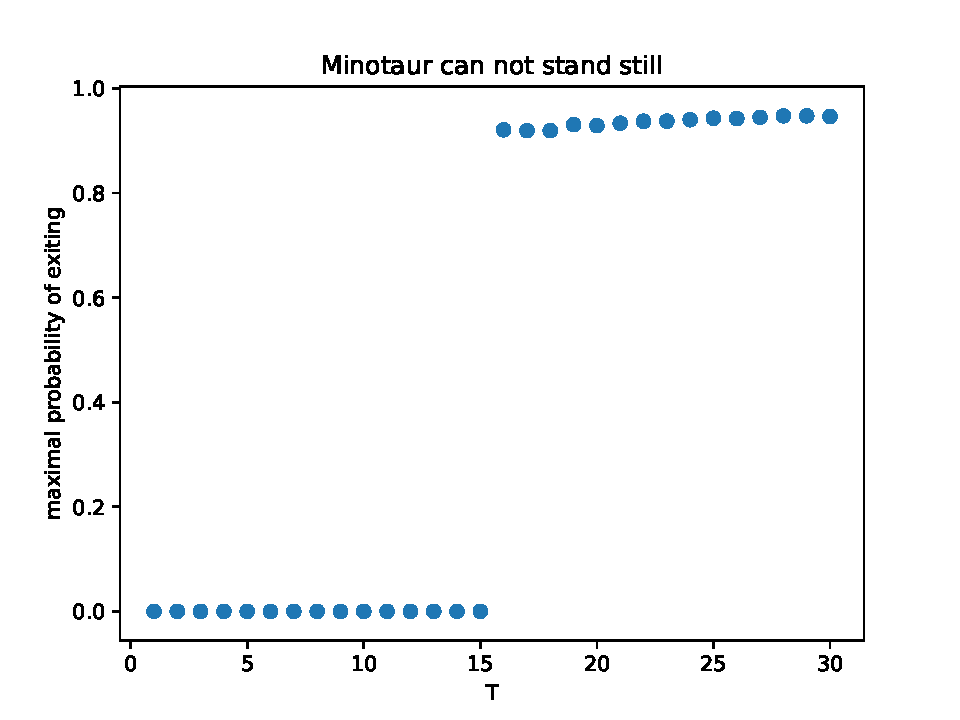
\includegraphics[width=.9\linewidth]{no_stand_still.pdf}
    \caption{Minotaur can not stand still.}
  \end{subfigure}%
  \begin{subfigure}{.5\textwidth}
    \centering
    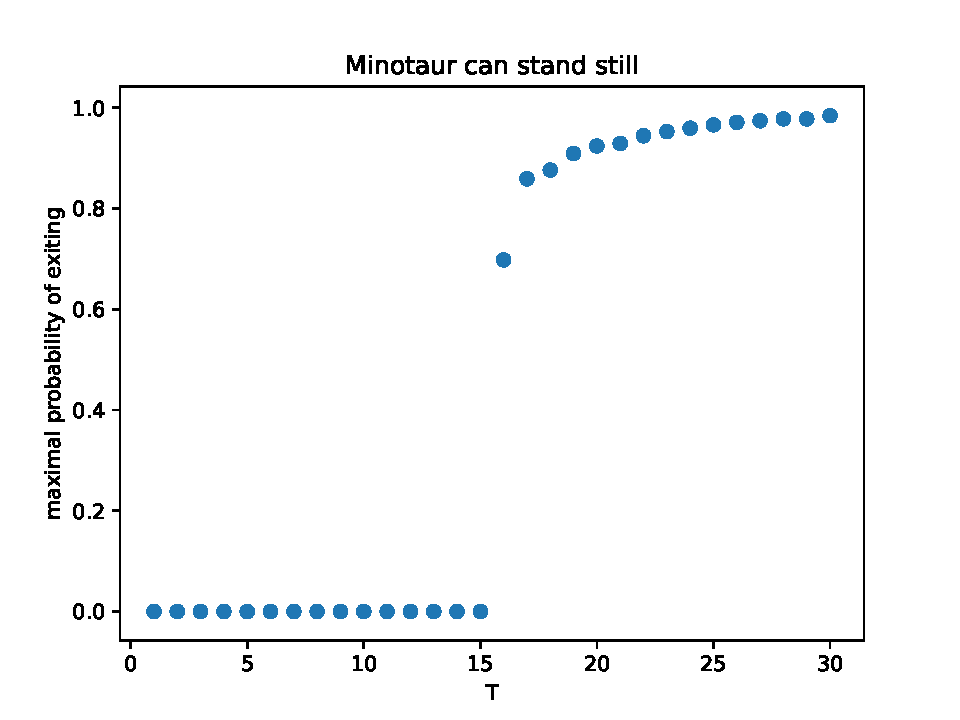
\includegraphics[width=.9\linewidth]{stand_still.pdf}
    \caption{Minotaur can stand still.}
  \end{subfigure}
  \caption{The probability of getting out alive the maze at T.}
  \label{fig:prob-getout-alive}
\end{figure}

For both cases, the exit probability for $T\leq 15$ is $0$. As the person need at least $15$ steps to arrive at exit even when there is not a minotaur.
When the minotaur is not allowed to stand still, the maximal probability for $T\geq 15$ is $1$. While in the other case, the maximal probability will gradually reach to 1 as $T$ increases.
When the minotaur stays in a position, the person will also keep still or move in an opposite direction to be as far as possible to the minotaur.
Thus, under this condition, the person tends to use more time to exit.
In other words, the maximal exiting probability with a standing still action will be a little bit less than that of the other case.

\subsection{Modify MDP with infinite time horizon}
Under this condition, the time horizon is no longer finite yet infinite.
The time $T$ is a random variable follows the geometric distribution:
\begin{equation*}
  P(t=T) = (1-p)^{t-1} p, \quad t \in \{1,2,\cdots\}
\end{equation*}
where $p=1 / 30 = 1 / \mathbb{E}(t)$. Therefore, it is unlikely to have a time $t \gg \mathbb{E}(t) = 30$.

Consider the expected reward over the random variable $T$:
% https://www.rapidtables.com/math/symbols/Statistical_Symbols.html
\begin{align*}
  \mathbb{E}[G_{T}]
    &= \mathbb{E}_{T, \tau}[r_T(s_T, a_T)] \\
    &= \lim_{T\rightarrow\infty} \mathbb{E}_{\tau}\left[\sum_{t=1}^{T} (1-p)^{t-1} r_t(s_t, a_t)\right] \\
    &= \lim_{T\rightarrow\infty} \mathbb{E}_{\tau}\left[\sum_{t=1}^{T} \lambda^{t-1} r_t(s_t, a_t)\right]
\end{align*}
where $\lambda = 1- p = 0.97$.

Therefore, we can re-formulate this problem as an infinite time horizon MDP with discounted rewards.

Other settings for this MDP are the same as before. And now we can use the value iteration(VI) algorithm to obtain the optimal policy.
After simulating 10000 games with the optimal policy obtained from VI, the estimated probability of exiting is $97.83\%$.
% Quesiton 2

% Quesiton 3
\section{Quesiton 3}
\subsection{Problem Formulation}

This problem is a discounted reinforcement learning problems

% state
\textbf{States:}

Consider the police location $S_p$ and the robber location $S_r$, can be represented
as a coordinate $(r, c)$, where $0 \leq r \leq 3$ is the row index and $0 \leq c \leq 3$
is the column index.

Therefore, the cardinality of the set $S_p$ and $S_r$ is 16 and
the cardinality the state of the problem $S = S_p \times S_r$ is 256.

\vspace{0.3cm}

% action
\textbf{Behavior policy and Actions:}

As the Q-learning is off-policy learning and the target policy (the policy being
learned) is optimal given that the behavior policy explores all (state, action) pairs
infinitely often.

Therefore, we use the radomized policy with the probability that is uniform
over actions as the behavior policy to generate the trajectory on infinite-time
horizon for learning.

\begin{align*}
  P(a \in A) &= \frac{1}{|A|}, \\
  \text{where} ~
  A &= \{\textup{Up},\textup{Down},\textup{Left},\textup{Right},\textup{StandStill}\}
\end{align*}
% Trans
\textbf{Transition probabilities:}

All transition is deterministic and therefore
\begin{equation*}
  p(s' | s, a) = 1
\end{equation*}

% reward
\textbf{Reward:}

As the transition is deterministic,
the reward can be formulated as a function of $r: S\times A \rightarrow S \rightarrow \mathbb{R}$.
\begin{equation*}
  r(s, a) = r(s') =
\begin{cases}
    -10 ,& \text{if } S_p = S_r\\
    1,   & \text{if } S_r = B\\
    0    & \text{otherwise}
\end{cases}
\end{equation*}
where $B$ is the bank location

% Q-learning
\subsection{Q-learning}

\textbf{Algorithm:}
\begin{steps}
  \item Initialize a Q-function with zeros
  \item Observe $(s_t, a_t, r_t, s_{t+1})$ under the randomized policy
  \item Update the Q-function with
  \begin{equation*}
    Q(s_t, a_t) = Q(s_t, a_t) + \alpha [r_t + \lambda\max_{b \in A} Q(s_{t+1}, b) - Q(s_t, a)]
  \end{equation*}
  where the learning rate $\alpha = 1 / n(s, a)$ and $n(s, a)$ is the number of visits
  of the $(s, a)$ pair
  \item Goto Step 2 and have $t = t + 1$.
\end{steps}

The plot of the value function over time at the initial state is shown in Figure
\ref{fig:q-learn-v0}.

We also plot the rolling average delta Q-function $|Q^{(t)} - Q^{(t-\Delta t)}|$ over time
to see if the Q-function converges in Figure \ref{fig:q-learn-delta-q}.
The matrix norm is Frobenius and
we take $\Delta t$ as 10000.


\begin{figure}
  \centering
  \begin{subfigure}{\textwidth}
    \centering
    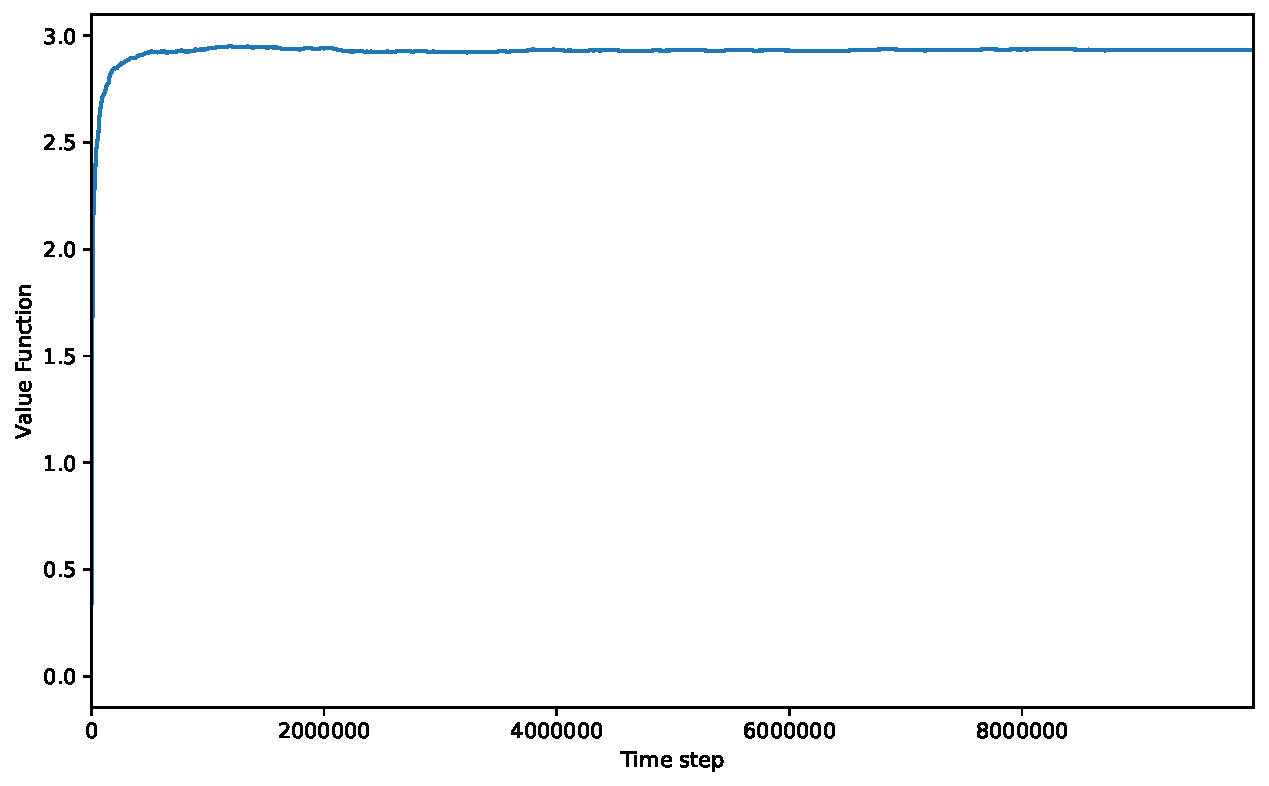
\includegraphics[width=\linewidth]{q_learn_v_fun_0.pdf}
    \caption{The value function over time at the initial state}
    \label{fig:q-learn-v0}
  \end{subfigure}

  \begin{subfigure}{\textwidth}
    \centering
    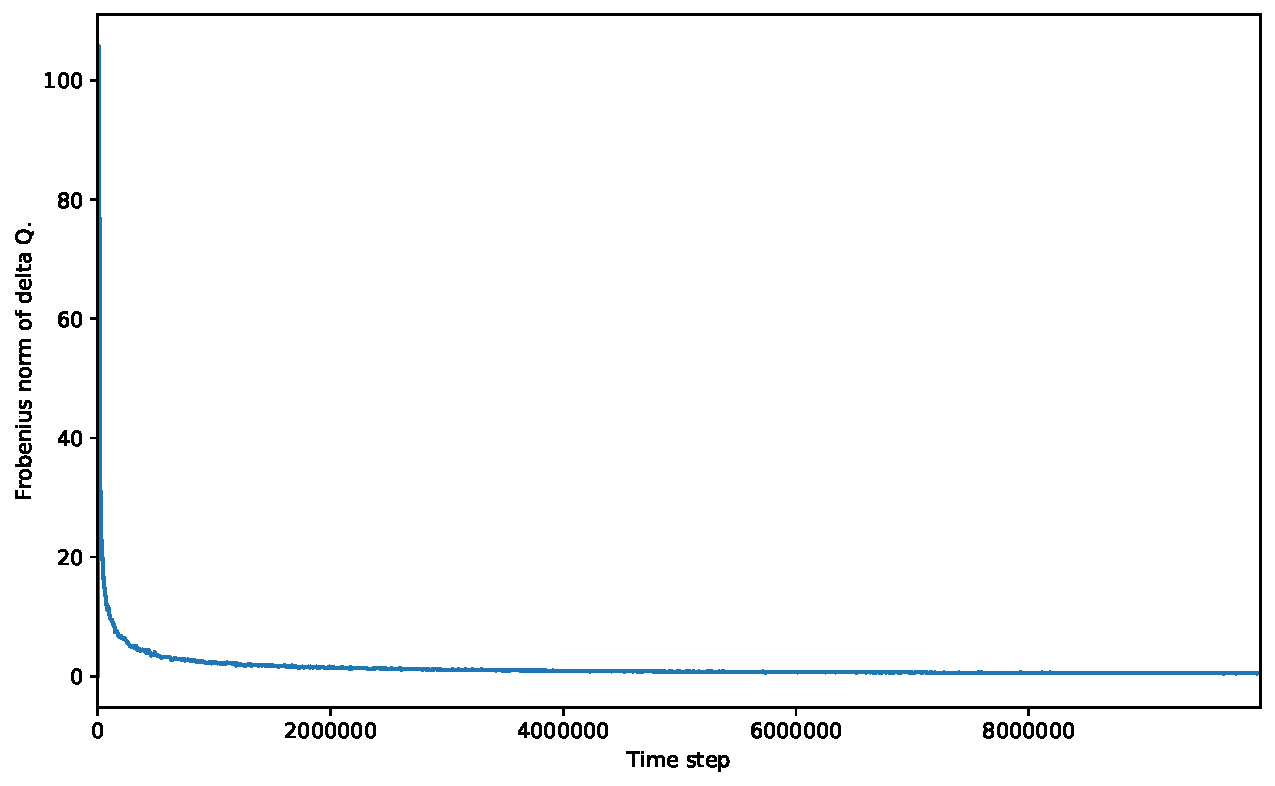
\includegraphics[width=\linewidth]{q_learn_norm_delta_q.pdf}
    \caption{The delta Q-function $|Q^{(t)} - Q^{(t-\Delta t)}|$ over time}
    \label{fig:q-learn-delta-q}
  \end{subfigure}
  \caption{Plots of the Q-learning process showing the convergence}
\end{figure}


% SASSA
\subsection{SASSA}

As we need $\epsilon$-greedy exploration, the RL problem remain the same except
the behavior policy.

\textbf{Behavior policy:}

The $\epsilon$-greedy policy is a mapping $\pi_b: S \rightarrow A $:

\begin{equation*}
  a =
  \begin{cases}
    \argmax_b Q(s, b) ,& \text{with probability} ~ 1 - \epsilon\\
    \text{uniform}(A) ,& \text{with probability} ~ \epsilon
  \end{cases}
\end{equation*}
depends on the current estimation of the Q-function.

\textbf{Algorithm:}
\begin{steps}
  \item Initialize a Q-function with zeros
  \item Observe $(s_t, a_t, r_t, s_{t+1}, a_{t+1})$ under the $\epsilon$-greedy
        policy based on current Q-function estimation.
  \item Update the Q-function with
\begin{equation*}
  Q(s_t, a_t) = Q(s_t, a_t) + \alpha [r_t + \lambda Q(s_{t+1}, a_{t+1}) - Q(s_t, a)]
\end{equation*}
  where the learning rate $\alpha = 1 / n(s, a)$ and $n(s, a)$ is the number of visits
  of the $(s, a)$ pair
  \item Goto Step 2 and have $t = t + 1$.
\end{steps}

The plot of the value function over time at the initial state is shown in Figure
\ref{fig:sassa-v0}.


We gave both the delta Q-function on normal scale and log scale as what we did
in Q-learning section.
However, we applied a rolling mean to the log scale plot as there are a lot
sudden changes.

Those sudden changes come from the $(s, a)$ pairs the SASSA algorithm visits
with the probability $\epsilon / |A|$ as the state-action pair is generally not
reached when applying the greedy behavior policy.

The results are shown in Figure \ref{fig:sassa-delta-q} and \ref{fig:sassa-delta-q-log}.

\begin{figure}
  \centering
  \begin{subfigure}{\textwidth}
    \centering
    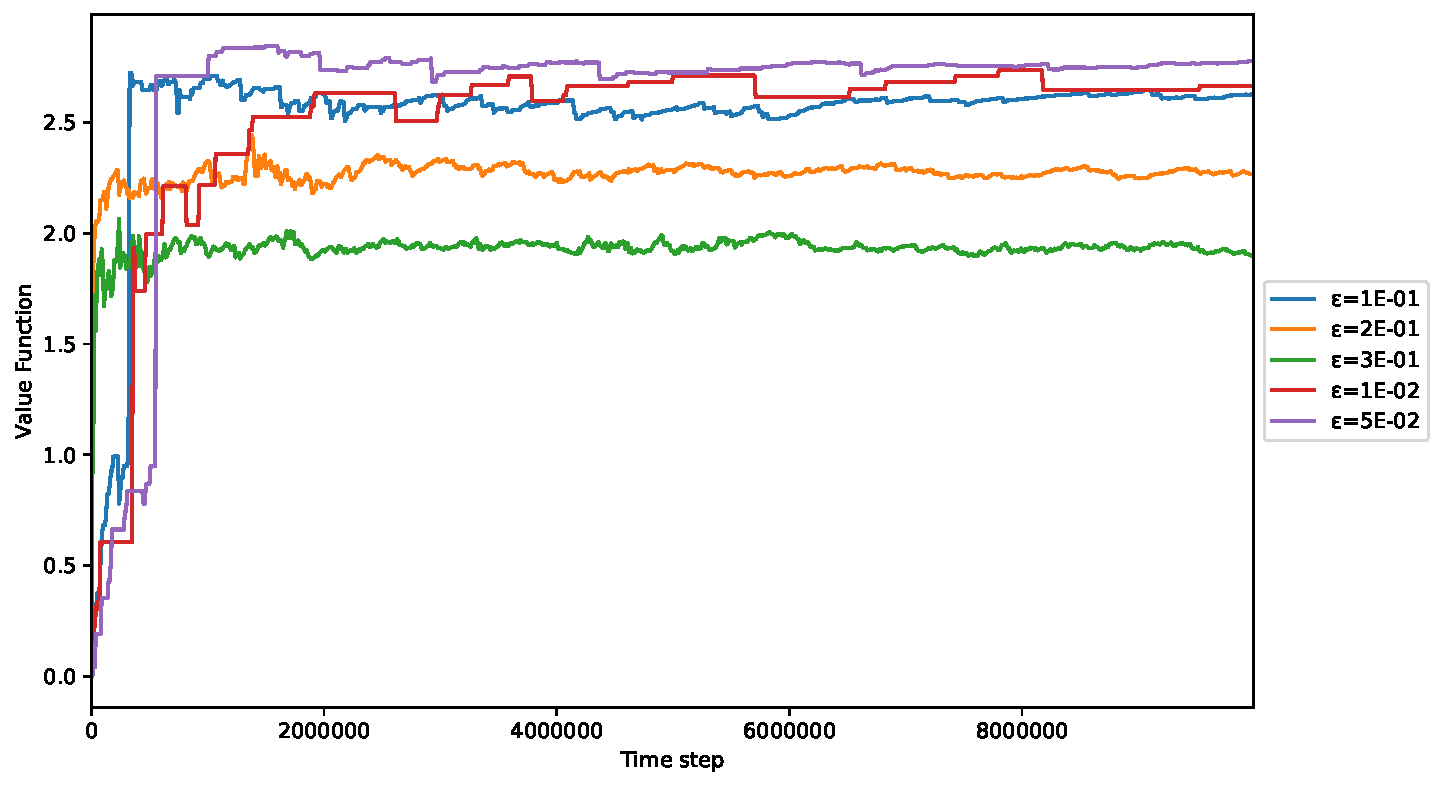
\includegraphics[width=.8\linewidth]{sassa_v_fun_0.pdf}
    \caption{The value function over time at the initial state}
    \label{fig:sassa-v0}
  \end{subfigure}
  \begin{subfigure}{\textwidth}
    \centering
    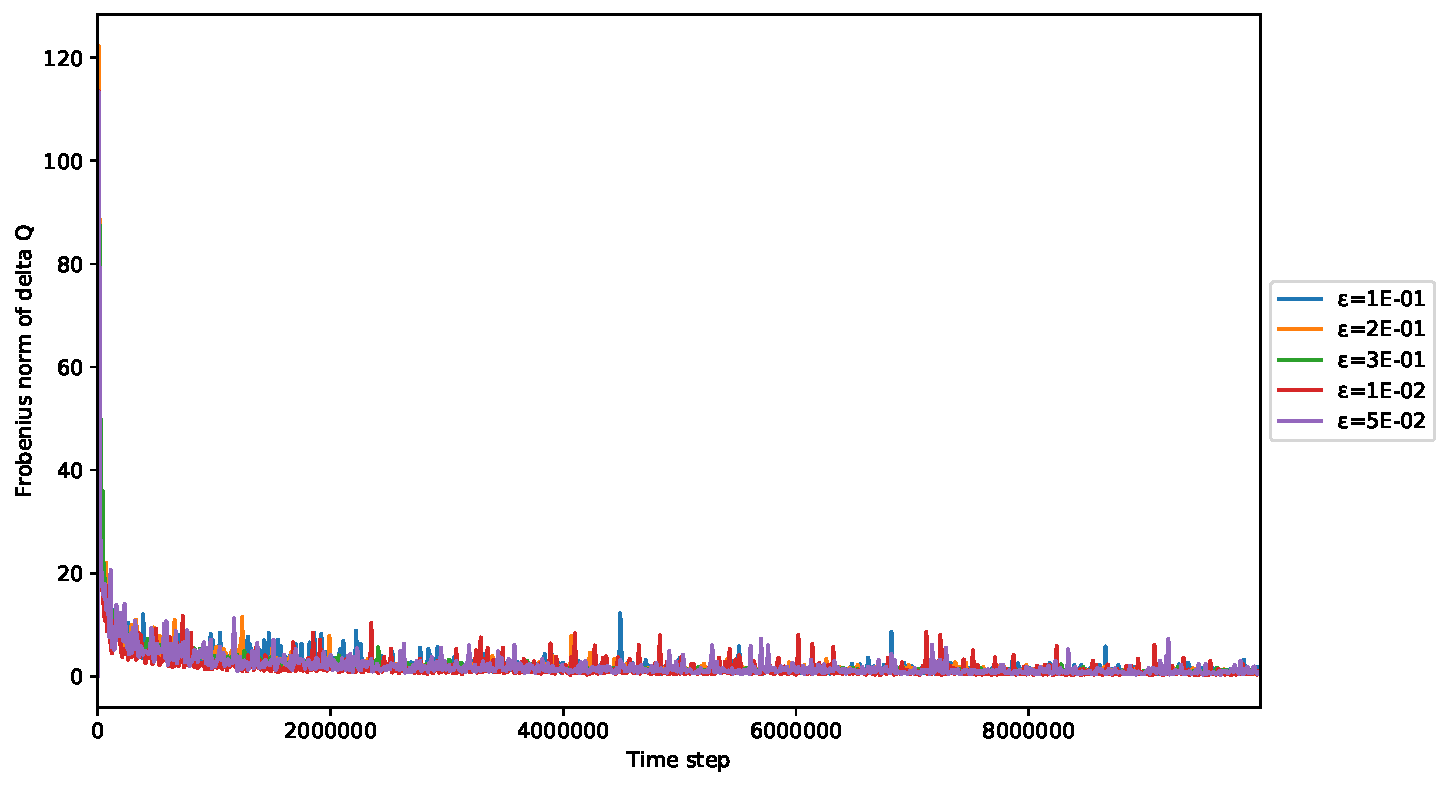
\includegraphics[width=.8\linewidth]{sassa_norm_delta_q.pdf}
    \caption{The delta Q-function $|Q^{(t)} - Q^{(t-\Delta t)}|$ over time}
    \label{fig:sassa-delta-q}
  \end{subfigure}
  \begin{subfigure}{\textwidth}
    \centering
    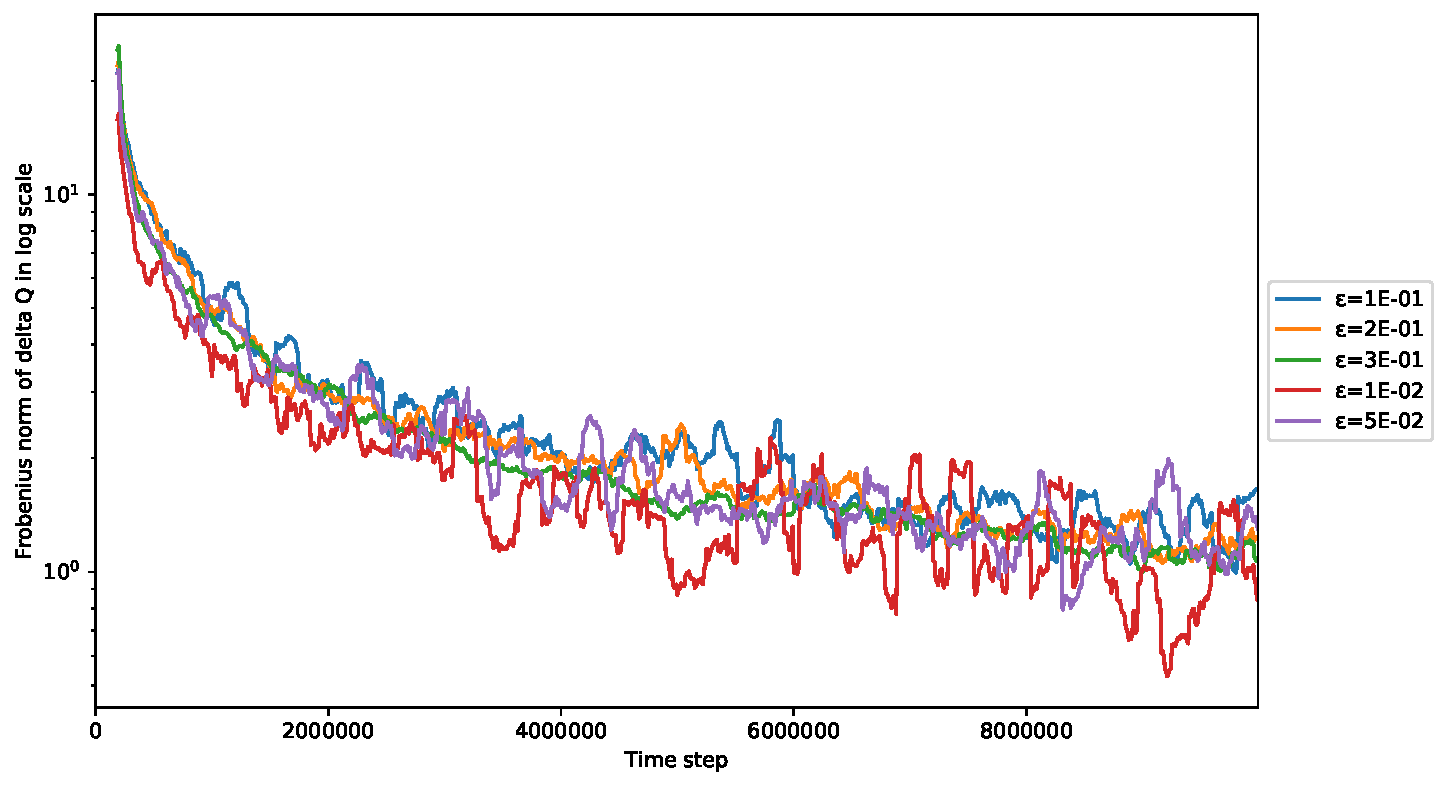
\includegraphics[width=.8\linewidth]{sassa_norm_delta_q_log.pdf}
    \caption{The rolling average delta Q-function $|Q^{(t)} - Q^{(t-\Delta t)}|$ over time on log scale}
    \label{fig:sassa-delta-q-log}
  \end{subfigure}
  \caption{Plots of the SASSA learning process showing the convergence}
\end{figure}


\end{document}
